\documentclass[]{article}

\usepackage{polski}
\usepackage[utf8]{inputenc}
%\usepackage[T1]{fontenc}

\usepackage[a4paper, total={6in, 8in}]{geometry}

\usepackage{graphicx}
\usepackage{float}
\usepackage{hyperref}
\hypersetup{
	colorlinks,
	citecolor=blue,
	filecolor=blue,
	linkcolor=blue,
	urlcolor=blue
}

%opening

\title{Aspekt inżynierski \\ Instrukcja instalacji i konfiguracji narzędzia}
\author{Mimkatz=\{Magda Waśniowska, Katarzyna Herba, Marcin Kania\}\\projekt realizowany w ramach Języki i Narzędzia Programowania 2 - grupa R}


\begin{document}

\maketitle

\section{Instrukcja aktualizacji danych}

By odtworzyć dane dotyczące ocen i ankiet niezbędne do poprawnego działania aplikacji trzeba:
\begin{enumerate}
	\item pobrać z bazy danych
	\item przepuścić przez program napisany w $C++$
	\item przepuścić przez program napisany w $R$
\end{enumerate}
W tej części opiszemy, jak te dane pobrać i w jaki sposób je przeczyścić.

\subsection*{Pobranie danych z bazy danych}
W celu pobrania danych z bazy danych należy najpierw połączyć się z bazą danych. Można to zrobić z poziomu terminalu (będąc na komputerze podłączonym do sieci wydziałowej) za pomocą następującej komendy:
\begin{verbatim}
rlwrap -ir sqlplus USER/PASSWORD@HOST:PORT/SERVICE_NAME
\end{verbatim}
\begin{itemize}
	\item $USER$ to nazwa użytkownika,
	\item $PASSWORD$ to hasło,
	\item $HOST$ to nazwa hosta,
	\item $PORT$ to numer portu,
	\item $SERVICE\_NAME$ to nazwa usługi.
\end{itemize}
Powyższa komenda wymaga zainstalowanego na maszynie użytkownik terminalowego klienta baz danych Oracle - SQL*Plus. Przykładowy widok uzyskiwania połączenia został przedstawiony na rysunku \ref{polaczenie_z_baza}.

\begin{figure}
	\centering
	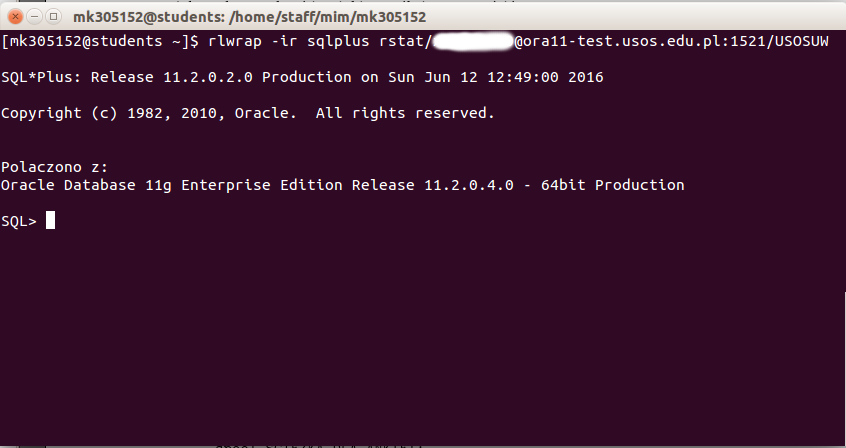
\includegraphics[width=80mm, height=50mm]{obrazki/logowanie-sql.png}
	\caption{Przykładowe połączenie z bazą danych (hasło wymazane na biało)}
	\label{polaczenie_z_baza}
\end{figure}

Będąc już połączonym z bazą danych należy wpisać następujące zapytania do niej:
\begin{itemize}
	\item w celu pobrania danych dotyczących ocen
	\begin{verbatim}
	set linesize 1000;
	spool SCIEZKA_DLA_OCEN;
	select KOD, PRZ_NAZWA, CDYD_KOD, NUMER_TERMINU, OCENA, OSOBA
	from rstat_oceny
	where jed_org_kod_biorca=10000000;
	spool off;
	\end{verbatim}
	\item w celu pobrania danych dotyczących ankiet
	\begin{verbatim}
	set linesize 1000;
	spool SCIEZKA_DLA_ANKIET;
	select KOD, PRZ_NAZWA, ZAJ_KOD, PROWADZACY, WARTOSC_ODPOWIEDZI,
	LICZBA_ODPOWIEDZI, TRESC_PYTANIA, CDYD_KOD
	from rstat_czestosci_ankiet
	where KOD like '%1000-%';
	spool off;
	\end{verbatim}
\end{itemize}

Należy w nich podmienić $SCIEZKA\_DLA\_OCEN$ na absolutną ścieżkę do pliku (czyli np. $\/home/dane/raw/oceny\_raw.txt$), do którego chcemy wgrać wyniki dla ocen. Analogicznie robimy z $SCIEZKA\_DLA\_ANKIET$.

Alternatywnie można uruchomić skrypt $data.sql$. Należy upewnić się, że skrypt znajduje się w katalogu, z którego łączymy się z bazą danych, a następnie wywołuje się go za pomocą polecenia:
\begin{verbatim}
@data.sql;
\end{verbatim}

\subsection*{Wstępne oczyszczenie danych za pomocą $jnpcleaner$}

Dane wyeksportowane z bazy danych nie są w postaci, którą można bezpośrednio zaimportować do programu R. Jest w nich wiele białych znaków i różnych znaków przystankowych uniemożliwiających podział danych na odpowiednią liczbę kolumn. Program $jnpcleaner$ służy do sparsowania wyjścia z bazy danych do formatu, który R może bezproblemowo odczytać.


\subsubsection*{Instrukcja kompilacji $jnpcleaner$}
Jeśli użytkownik nie posiada pliku wykonywalnego $jnpcleaner$, to powinien skompilować go używając źródeł. W tym celu należy:

\begin{enumerate}
	\item otworzyć terminal,
	\item przejść do katalogu zawierającego kod źródłowy $src$ aplikacji $jnpcleaner$,
	\item wywołać w terminalu z poziomu wyżej wymienionego katalogu polecenie $cmake ..$.,
	\item wywołać teraz $make$.
\end{enumerate}

W przypadku poprawnego wykonaniu powyższych czynności w katalogu $src$ pojawi się plik wykonywalny $jnpcleaner$.

Aby użytkownik mógł skompilować $jnpcleaner$ zgodnie z wyższą metodą, musi posiadać odpowiednie narzędzie tzn. kompilator oraz program $cmake$. Użytkownicy systemów z rodziny $UNIX$ nie powinni mieć problemu z tym, gdyż zazwyczaj kompilator taki jest udostępniony wraz z dystrybucją systemu, więc muszą jedynie pobrać z sieci $cmake$ (jest darmowy).

W przypadku użytkowników systemu $Windows$, polecamy zainstalować pakiet $Cygwin$ - za jego pomocą można zainstalować kompilator $C++$. Sugerowany kompilator to gcc w wersji 4.9.2. Również, jak w przypadku systemów rodziny $UNIX$, należy pobrać program $cmake$.

\subsubsection*{Instrukcja używania $jnpcleaner$}

Program $jnpcleaner$ uruchamia się komendą
\begin{verbatim}
 ./jnpcleaner
\end{verbatim}
z poziomu terminalu. Aby program poprawnie zadziałał należy mu podać następujące argumenty:

\begin{itemize}
	\item jeśli przetwarzamy dane dotyczące ocen i ankiet
	\begin{verbatim}
	./jnpcleaner "both" "GradesInPath" "GradesOutPath"
	"QuestionsInPath" "QuestionsOutPath";
	\end{verbatim}
	\item jeśli przetwarzamy tylko dane dotyczące ocen
	\begin{verbatim}
	./jnpcleaner "grades" "GradesInPath" "GradesOutPath";
	\end{verbatim}
	\item jeśli przetwarzamy tylko dane dotyczące ankiet
	\begin{verbatim}
	./jnpcleaner "questions" "QuestionsInPath" "QuestionsOutPath";
	\end{verbatim}
\end{itemize}
gdzie $GradesInPath$, $GradesOutPath$, $QuestionsInPath$ i $QuestionsOutPath$ to zmienne, za które należy podstawić absolutne ścieżki odpowiednio do: 
\begin{itemize}
	\item pliku zawierającego surowe dane z bazy danych dotyczące ocen,
	\item pliku (niekoniecznie utworzonego) mającego zawierać oczyszczone dane dotyczące ocen,
	\item pliku zawierającego surowe dane z bazy danych dotyczące ankiet,
	\item pliku (niekoniecznie utworzonego) mającego zawierać oczyszczone dane dotyczące ankiet.
\end{itemize}

Przykładowe wywołanie to:
\begin{verbatim}
./jnpcleaner "both" "/home/dane/grades_raw.txt" "/home/dane/grades_clean.txt"
"/home/dane/questions_raw.txt" "/home/dane/questions_clean.txt"
\end{verbatim}

Na systemach typu $Windows$ za terminal służy np. $cmd.exe$, wówczas zamiast 
\begin{verbatim}
./jnpcleaner
\end{verbatim}
należy użyć komendy 
\begin{verbatim}
jnpcleaner.exe
\end{verbatim}

Alternatywnie można wywołać plik bashowy $clean.sh$, po wcześniejszym podmienieniu ścieżek docelowych w nim. Nomenklatura zmiennych dla ścieżek jest dokładnie taka sama, jak wyżej. Po poprawnym podmienieniu $clean.sh$ wywołuje się komendą $./clean.sh$. W przypadku systemu $Windows$ należy skorzystać w udostępnionego w ramach środowiska $Cygwin$ terminalu i w nim wywołać skrypt.

\subsection*{Wtórne oczyszczenie danych w $R$}

Program $oczyszczenie\_danych.R$ służy do:
\begin{itemize}
	\item zastąpienia encji zawierających oceny uzyskane przez studenta w różnych terminach (z tego samego przedmiotu) przez jedną encją z ostateczną oceną,
	\item usunięcia danych nieużywanych w aplikacje (oceny z przedmiotów prowadzonych poza MIM UW),
	\item wyfiltrowania roczników od semestru letniego 2008 włącznie,
	\item rozdzielenia przedmiotów, które mają taką samą nazwę ale inny kod,
	\item usunięcia namiarowych białych znaków występujących w danych,
	\item usunięcia danych o przedmiotach o których wiadomo, że nie są już prowadzone przez MIM UW.
\end{itemize}
Aby użyć programu, należy otworzyć go w programie $RStudio$ i pobrać bibliotekę $plyr$ poleceniem 
\begin{verbatim}
install.packages("plyr").
\end{verbatim} 
Następnie należy w pliku uzupełnić ścieżki do plików, znajdujące się w pierwszych linijkach programu: 
\begin{verbatim}
path_read
\end{verbatim}
to ścieżka, do danych uzyskanych po przepuszczeniu danych pobranych z bazy danych przez program jnpcleaner,
\begin{verbatim}
path_write
\end{verbatim}
to ścieżka, pod którą zostaną zapisane uzyskane w ten sposób dane do aplikacji. Po ustawieniu ścieżek należy zaznaczyć cały kod $oczyszczenie\_danych.R$ i uruchomić go komendą $Run$, znajdującą się w prawym górnym rogu aplikacji.
%jeżeli aplikacja nie korzysta bezpośrednio ze zdalnego źródła danych ale robi lokalną kopię, należy dołączyć instrukcję w jaki sposób dane aktualizować, jaki skrypt uruchomić, z jakimi parametrami narzędzia


\section{Instrukcja instalacji $R$ i konfiguracji aplikacji $Shiny$}
W celu uruchomienia naszej aplikacji trzeba posiadać odpowiednią wersję środowiska programowania $R$ oraz stosowne biblioteki. W tej części podamy wymagane programy, biblioteki oraz opiszemy sposób konfiguracji aplikacji, by działała na maszynie użytkownika. Sugerujemy, aby użytkownik zainstalował program $RStudio$, gdyż jest to bardzo dobre środowisko do pracy w języku $R$.


%należy dołączyć instrukcję w jaki sposób dane narzędzie instalować na innym komputerze (co trzeba wgrać, jakie są zależności) i jak uruchomić

\begin{enumerate}
	\item Zainstalować program $R$ (wersja minimum 3.3.0).
	\item W programie $R$ zainstalować następujące biblioteki:
	\begin{verbatim}
		library(shiny)
		library(ggplot2)
		library(plyr)
		library(xtable)
		library(reshape2)
	\end{verbatim}
	
	\item W obu plikach \textbf{server.R} oraz \textbf{ui.R} uzupełnić ścieżki prowadzące do danych (pierwsze linie kodu). Przykładowo:
	
	\begin{verbatim}
	ankiety_path <- "home/user/Desktop/ankiety_clean.txt"
	oceny_path <- "/home/user/Desktop/oceny.csv"
	\end{verbatim}
	
\end{enumerate}
Warto tu zauważyć, że ścieżka $oceny\_path$ (w plikach \textbf{server.R} i \textbf{ui.R}) musi być taka sama jak $path\_write$ (w pliku oczyszczenie\_danych.R).

\section{Instrukcja obsługi}

%należy dołączyć instrukcję jak korzystać z narzędzia

Aplikacja pozwala na porównywanie udziału poszczególnych ocen w końcowych wynikach z danego przedmiotu na przestrzeni ostatnich lat. Prezentowane oceny są ostatecznymi jakie otrzymała dana osoba tzn. jeśli student X miał z przedmiotu Y oceny w terminach 1, 2 i 3 to w aplikacji została wykorzystana tylko ocena z terminu numer 3.

\begin{itemize}
	\item 
	W pierwszym kroku użytkownik wybiera przedmiot do analizy dostępny spośród rozwijanej listy przedmiotów prowadzonych przez jednostkę MIM UW (\ref{przedmiot}).
	\begin{figure}[H]
		\centering
		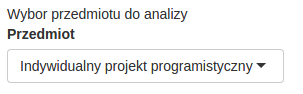
\includegraphics[width=55mm,height=20mm]
		{obrazki/przedmiot.png}
		\caption{Zrzut fragmentu ekranu prezentujący wybór przedmiotu}
		\label{przedmiot}
	\end{figure}
	
	\item 
	W drugim kroku należy wskazać cykl/e dydaktyczne, których będą dotyczyły prezentowane dane (\ref{cykl}). Dodatkowo użytkownik ma do wyboru dwa przyciski "Zaznacz wszystkie cykle" i "Odznacz wszystkie cykle", które odpowiednio zaznaczają i odznaczają wszystkie możliwe do wyboru cykle dydaktyczne. Dodatkowo użytkownik będzie miał do wyboru tylko te lata w których prowadzony był przedmiot wybrany w kroku numer 1.
	\begin{figure}[H]
		\centering
		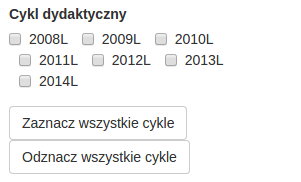
\includegraphics[width=60mm,height=35mm]
		{obrazki/cykl.png}
		\caption{Zrzut fragmentu ekranu prezentujący wybór cyklu dydaktycznego}
		\label{cykl}
	\end{figure}
	
	\item 
	Prezentacja wykresów odbywa się w dwa różne sposoby albo na jednym (\ref{wykres_razem}) albo w podziale na cykle (\ref{wykres_osobno}). Opcja wyboru wykresu znajduje się w panelu sterowania po lewej stronie aplikacji (\ref{na_jednym}).
	\begin{figure}[H]
		\centering
		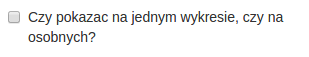
\includegraphics[width=60mm,height=15mm]
		{obrazki/na-jednym.png}
		\caption{Zrzut fragmentu ekranu prezentujący pytanie dotyczące prezentacji wykresu}
		\label{na_jednym}
	\end{figure}
	
	\item
	Użytkownik ma do wyboru cztery różne zakładki (\ref{wynik}). Pierwsza z nich domyślnie włączona przedstawia wyżej omówione wykresy. Druga "Ankiety-Wykres" prezentuje wykres dotyczący danych z ankiet (\ref{wykres_ankiet}). Dwie kolejne są to zakładki z tabelami, pierwsza (\ref{tabela_oceny}) zawiera tabelę z danymi dotyczącymi ocen natomiast druga (\ref{tabela_ankiety}) - ankiet. Dane prezentowane w tabelach są tymi samymi danymi, które są użyte do wygenerowania wykresów.
	\begin{figure}[H]
		\centering
		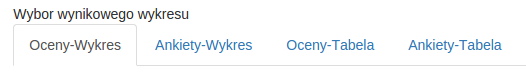
\includegraphics[width=120mm]
		{obrazki/wynik.png}
		\caption{Zrzut fragmentu ekranu prezentujący dostępne zakładki}
		\label{wynik}
	\end{figure}
	
	\item Wykres prezentujący wyniki ankiet (\ref{wykres_ankiet}) dotyczy przedmiotu wybranego w kroku pierwszym (\ref{przedmiot}) oraz cykli dydaktycznych (\ref{cykl}) z kroku drugiego. Dodatkowo użytkownik powinien wybrać pytanie, dla którego chce zobaczyć wyniki. W panelu sterowania po lewej stronie służy do tego rozwijana lista (\ref{pytanie}). 
	\begin{figure}[H]
		\centering
		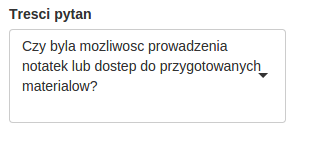
\includegraphics[width=60mm,height=30mm]
		{obrazki/pytanie.png}
		\caption{Zrzut fragmentu ekranu prezentujący wybór pytania ankiety}
		\label{pytanie}
	\end{figure}
	
\end{itemize}

\begin{figure}[H]
	\centering
	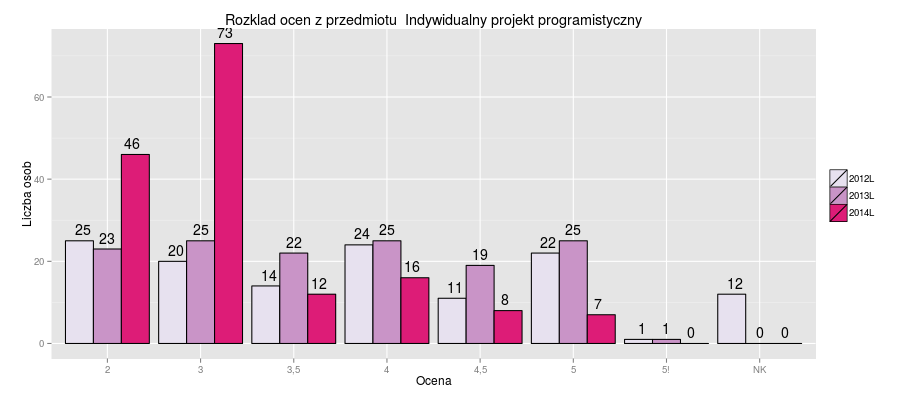
\includegraphics[width=100mm, height=60mm]
	{obrazki/wykres-razem.png}
	\caption{Wykres typu 1}
	\label{wykres_razem}
\end{figure}

\begin{figure}[H]
	\centering
	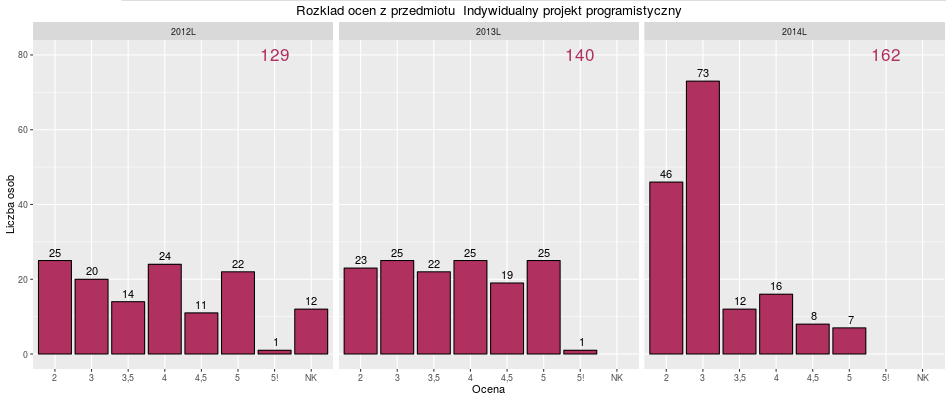
\includegraphics[width=100mm,height=60mm]
	{obrazki/wykres-oceny-wiele.png}
	\caption{Wykres typu 2}
	\label{wykres_osobno}
\end{figure}

\begin{figure}[H]
	\centering
	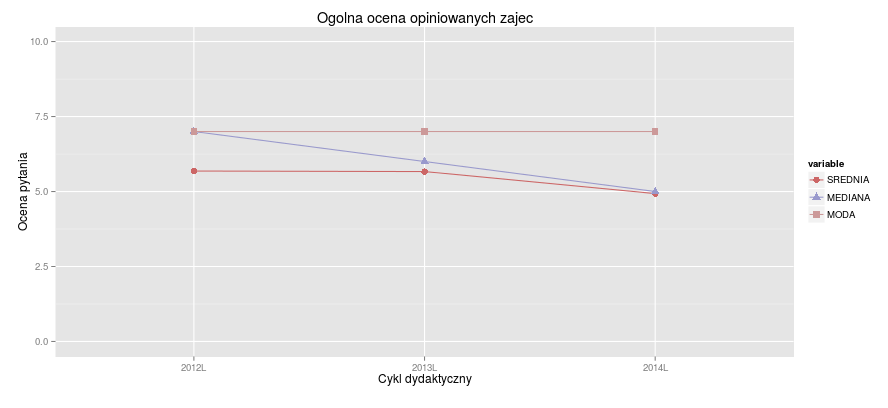
\includegraphics[width=100mm, height=60mm]{obrazki/wykres-ankieta.png}
	\caption{Wykres danych z ankiet}
	\label{wykres_ankiet}
\end{figure}

\begin{figure}[H]
	\centering
	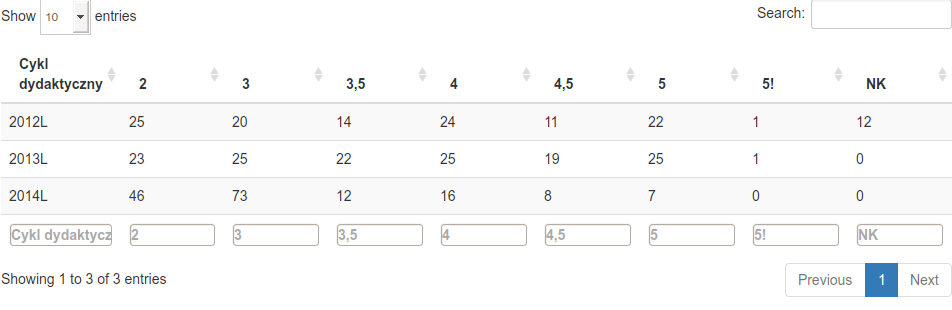
\includegraphics[width=100mm, height=50mm]{obrazki/oceny_tabela.png}
	\caption{Tabelarne zestawienie ocen z przedmiotów na tle cyklów dydaktycznych}
	\label{tabela_oceny}
\end{figure}

\begin{figure}[H]
	\centering
	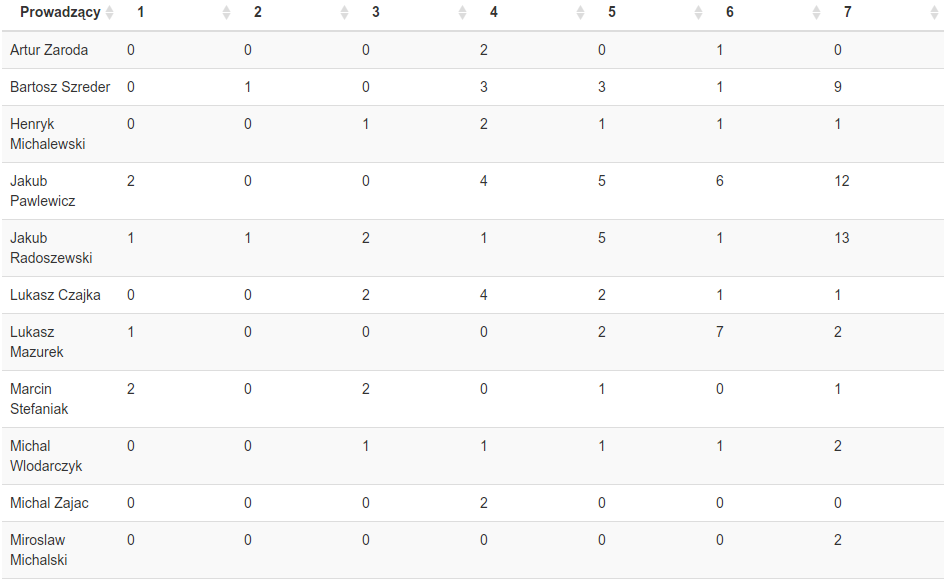
\includegraphics[width=120mm, height=60mm]{obrazki/oceny-tabela.png}
	\caption{Tabelarna zestawienie wyników konkretnego pytania z ankiet na tle prowadzących}
	\label{tabela_ankiety}
\end{figure}


\end{document}
